\chapter{HIV NEUTRALIZING ANTIBODIES IN HIV NA�VE DONORS}
\section{Introduction}
\begin{figure}
   \centering
   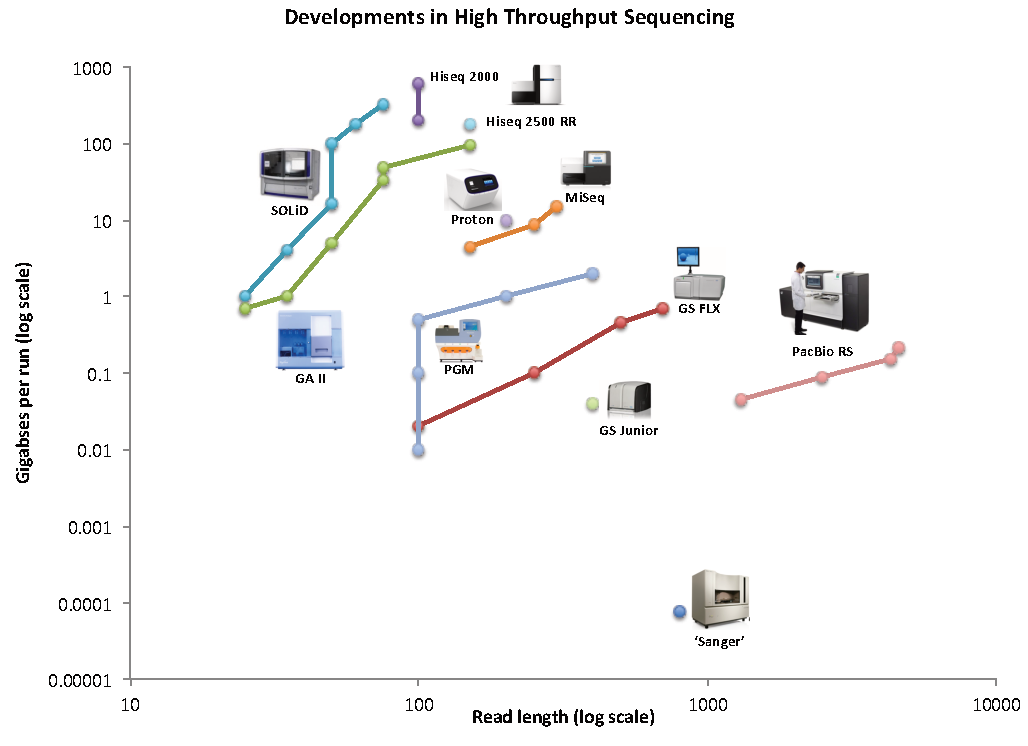
\includegraphics[width=.9\linewidth]{images/chapter3/figure3_1.pdf} % requires the graphicx package
   \caption[Current Sequencing Technologies]{Current sequencing technologies. On the x-axis is the current read length for each sequencing platform. The y-axis is the bases per run. Each point is a new iteration of that platforms sequencing read length and coverage. HiSeq has the most coverage with relatively short read lengths. Figure adapted from \citep{developmentinNGS:2012bs} }
   \label{fig:figure3_1}
\end{figure}

\begin{table}[t]
\centering
\resizebox{.99\linewidth}{!}{
\begin{tabular}{lllrrS[table-format=3.2]}
\toprule
\textbf{Platform}   & \textbf{Instrument}      & \textbf{Year} & \textbf{Reads per run} & \textbf{Read length (mode or average)} & \textbf{Bases per run (gigabases)} \\
\midrule
Sanger & 3730xl          & ND   & 96            & 800                           & 0.0000768                 \\
454        & GS20            & 2005 & 200,000        & 100                           & 0.02                      \\
454        & GS FLX          & 2007 & 400,000        & 250                           & 0.1                       \\
454        & GS FLX Titanium & 2009 & 1,000,000       & 500                           & 0.45                      \\
454        & GS FLX+         & 2011 & 1,000,000       & 700                           & 0.7                       \\
454        & GS Junior       & 2010 & 100,000        & 400                           & 0.04                      \\
IonTorrent & PGM 314 chip    & 2011 & 100,000        & 100                           & 0.01                      \\
IonTorrent & PGM 316 chip    & 2011 & 1,000,000       & 100                           & 0.1                       \\
IonTorrent & PGM 318 chip    & 2011 & 5,000,000       & 100                           & 0.5                       \\
IonTorrent & PGM 318 chip    & 2012 & 5,000,000       & 200                           & 1.0                         \\
IonTorrent & PGM 318 chip V2 & 2013 & 5,000,000       & 400                           & 2.0                         \\
IonTorrent & Proton PI       & 2012 & 50,000,000      & 200                           & 10.0                        \\
Illumina   & GA              & 2008 & 28,000,000      & 35                            & 1.0                         \\
Illumina   & GA II           & ND   & 100,000,000     & 50                            & 5.0                         \\
Illumina   & GAIIx           & 2009 & 440,000,000     & 75                            & 33.0                        \\
Illumina   & GAIIx           & 2011 & 640,000,000     & 75                            & 48.0                        \\
Illumina   & GAIIx           & 2012 & 640,000,000     & 150                           & 95.0                        \\
Illumina   & HiSeq 2000      & 2010 & 2,000,000,000    & 100                           & 200.0                       \\
Illumina   & HiSeq 2000      & 2011 & 3,000,000,000    & 100                           & 600.0                       \\
Illumina   & HiSeq 2500 RR   & 2012 & 600,000,000     & 150                           & 180.0                       \\
Illumina   & MiSeq           & 2011 & 30,000,000      & 150                           & 4.5                       \\
Illumina   & MiSeq           & 2012 & 30,000,000      & 250                           & 8.5                       \\
Illumina   & MiSeq           & 2013 & 30,000,000      & 300                           & 15.0                        \\
SOLiD      & 3               & ND   & 320,000,000     & 50                            & 16.0                        \\
SOLiD      & 4               & ND   & 2,000,000,000    & 50                            & 100.0                       \\
SOLiD      & 5500xl          & 2011 & 3,000,000,000    & 60                            & 180.0                       \\
SOLiD      & 5500xl W        & 2013 & 3,000,000,000    & 75                            & 320.0                       \\
PacBio     & RS C1           & 2011 & 36,000         & 1,300                          & 0.045                     \\
PacBio     & RS C2           & 2012 & 36,000         & 2,500                          & 0.090                     \\
PacBio     & RS C2 XL        & 2012 & 36,000         & 4,300                          & 0.155                     \\
PacBio     & RS II C2 XL     & 2013 & 47,000         & 4,600                          & 0.216                    \\
\bottomrule
\end{tabular}}
\caption[Current HTS Sequencing Platforms]{Figure adapted from \citep{developmentinNGS:2012bs}}
\label{tab:table3_1}
\end{table}